





\documentclass[12pt,letterpaper,notitlepage]{article}
\usepackage{graphicx}
\usepackage{epsfig,epsf}
\usepackage{epstopdf}
\usepackage{curves}
\usepackage{hyperref}
% The following packages are important as they allow to write certain mathematical expressions.
\usepackage{amsmath}
\usepackage{amssymb}
\usepackage{color}
% To write a code in a LaTeX document you need:
\usepackage{listings}
\definecolor{dkgreen}{rgb}{0,0.6,0}
\definecolor{dkblue}{rgb}{0,0.0,0.6}
\definecolor{dkred}{rgb}{0.9,0.0,0.1}
%% Own definitions:
\newcommand{\BEq}{\begin{eqnarray}}
\newcommand{\EEq}{\end{eqnarray}}
\newcommand{\BEqn}{\begin{eqnarray*}}
\newcommand{\EEqn}{\end{eqnarray*}}
\newcommand{\BM}{\begin{subequations}}
\newcommand{\EM}{\end{subequations}}
\newcommand{\BEqM}{\begin{subequations}\begin{eqnarray}}
\newcommand{\EEqM}{\end{eqnarray}\end{subequations}}
\newcommand{\Bitem}{\begin{itemize}}
\newcommand{\Eitem}{\end{itemize}}
\newcommand{\Ben}{\begin{enumerate}}
\newcommand{\Een}{\end{enumerate}}
%% Greek letters:
\renewcommand{\a}{\alpha}
\renewcommand{\b}{\beta}
\newcommand{\D}{\Delta}
%% Colors:
\newcommand{\TB}[1]{\textcolor{blue}{#1}}
\newcommand{\TR}[1]{\textcolor{red}{#1}}
\newcommand{\bm}[1]{\mbox{\boldmath $#1$}}
\newcommand{\non}{\nonumber\\}
%% Some simplified expressions:
\def\eps{\varepsilon}
\def\r{\right}
\def\l{\left}
\def\p{\partial}
\def\d{\delta}
\newcommand{\ta}{\mbox{$\theta$}}
\newcommand{\ve}{\mbox{${\cal E}$}}
\newcommand{\etab}{\bar{\eta}}
\newcommand{\sg}{\tilde{\sigma}}
\newcommand{\tap}{\mbox{$\theta'$}}
\newcommand{\tta}{\mbox{$\tilde{\theta}$}}
\newcommand{\ttap}{\mbox{$\tilde{\theta}'$}}
\newcommand{\taz}{\mbox{$\theta_0$}}
\newcommand{\phip}{\mbox{$\phi'$}}
\newcommand{\tphi}{\mbox{$\tilde{\phi}$}}
\newcommand{\tphip}{\mbox{$\tilde{\phi}'$}}
\newcommand{\ty}{\mbox{$\tilde{y}$}}
\newcommand{\gb}{\mbox{$\bar{\gamma}$}}
\newcommand{\gone}{\mbox{$\gamma_1$}}
\newcommand{\gtwo}{\mbox{$\gamma_2$}}
\newcommand{\phiz}{\mbox{$\phi_0$}}
\newcommand{\Nf}{\mbox{$N_f$}}
\newcommand{\Nv}{\mbox{$N_v$}}
\newcommand{\qt}{\mbox{$\tilde{q}$}}
\newcommand{\qa}{\mbox{$q_\alpha$}}
\newcommand{\tqa}{\mbox{$\tilde{q}_\alpha$}}
\newcommand{\dqa}{\mbox{$\delta q_\alpha$}}
\newcommand{\pqa}{\mbox{$\partial_{u} q_\alpha$}}
\newcommand{\pqta}{\mbox{$\partial_{u} \tilde{q}_\alpha$}}
\newcommand{\pdqa}{\mbox{$\partial_{u}\delta q_\alpha$}}
\newcommand{\sn}{\mbox{${\rm sn}$}}
\newcommand{\cn}{\mbox{${\rm cn}$}}
\newcommand{\dn}{\mbox{${\rm dn}$}}
\newcommand{\cd}{\mbox{${\rm cd}$}}
%%% Creation, destruction operators:
\newcommand{\cks}{\mbox{$c_{{\bf k},\sigma}$}}
\newcommand{\cksd}{\mbox{$c_{{\bf k},\sigma}^\dagger$}}
\newcommand{\cku}{\mbox{$c_{{\bf k},\uparrow}$}}
\newcommand{\ckd}{\mbox{$c_{-{\bf k},\downarrow}$}}
\newcommand{\ckud}{\mbox{$c_{{\bf k},\uparrow}^\dagger$}}
\newcommand{\ckdd}{\mbox{$c_{-{\bf k},\downarrow}^\dagger$}}

\begin{document}

\lstset{language=Fortran,tabsize=4,numbers=left,numberstyle=\tiny,basicstyle=\ttfamily\small\color{dkblue},stringstyle=\ttfamily\color{blue},keywordstyle=\rmfamily\color{dkred}\bfseries\emph,backgroundcolor=\color{white},commentstyle=\color{dkgreen}}




\title{%
	Continued Fraction Approach to Cumulative Density Function \\
\large Computional Physics - Phys 562}
\author{Benjamin Deutsch  \\
Department of Physics\\
California State University Long Beach}
\date{\today }

  
\maketitle



\begin{abstract}
Here we will utilize the Fortran 95 Programming environment to execute a series of functions; complex continued fractions, to assist in plotting the error function. This result will then be placed into the cumulative density function, ${F(x, \mu, \sigma^2) =\frac{1}{2}} \left[1+ erf \left( \frac{x -\mu}{\sigma\sqrt{2}} \right) \right]$. With constants ${\sigma}$ = 1.5 and ${\mu} = 2$ between -4, 8. The output was saved as a \textbf{.dat} extension and plotted.    
\end{abstract}

\section{Introduction}

The normal cumulative density finds many uses, as a simple probability distribution resolving from less than or equal to the given number of occurrences; (x). If however the function happens to be continuous, the area under the slope will complement the standard probability density plot used most commonly in statistic. While very rudimentary, the idea can extend to many areas of physics namely quantum mechanics, the field where many discrete events are better seen as a whole, or distribution. A need to create a program that plots the function arises from the extremely labor intensive calculations of finding each of these points. This is only compounded by the error function which is included in the formula. While Fortran contains an intrinsic function for this, there is exercise found in allowing the students to create their own code for the error function. This itself can be approached in a variety of ways, however making use of the recent lectures we find advantage in the notes taken on the continued fraction series, as a way to approximate the error function value. 


\section{The Math and Theory}

For the assignment we are asked to plot the normal cumulative,

	\begin{equation}
	{F(x, \mu, \sigma^2) =\frac{1}{2}} \left[1+ erf \left( \frac{x -\mu}{\sigma\sqrt{2}} \right) \right]	
	\end{equation}
\\
The error function can expanded into a complex series as; 
\\
	\begin{equation}
	w(z) = \frac{i}{\sqrt{\pi}}\frac{1}{z-}\frac{\frac{1}{2}}{z-}\frac{1}{z-}\frac{\frac{3}{2}}{z-}....,
	\end{equation}	
\\
Rewritten. We can then approximate this result with a set of functions; 
\\
	\begin{equation}
		w(z)=e^{-z^{2}}\left(1+\frac{2i}{\sqrt{\pi}}\int_{0}^{z}e^{t^{2}}dt\right)=e^{-z^{2}}{erfc}(-iz)
	\end{equation}
\\
	\begin{equation}
	erfc z={\frac{2}{\sqrt{\pi}}\int_{z}^{\infty}e^{-t^{2}}dt=1-erf} z	
	\end{equation}
\\
	\begin{equation}
	erf(z) = z=\frac{2}{\sqrt{\pi}}\int_{0}^{z}e^{-t^{2}}
	\end{equation}
We have clearly defined a complementary function pathway which has absorbed the complex terms and made it relatively effortless to input into the Fortran environment.  

\section{The code}

For all Fortran code we must begin with the variables, all terms used here in this program are define in the heading, as real, or integer. Some values such as $\sigma$ and $\mu$ have have given constant values; 1.5 and 2, respectively. Some calculations have occurred here in the heading as well such a definition of step size.  

This code differs from previous code by the use of the \textbf{contains} command, found near the end of the program. This enables the writer to create unique functions that can be called up from the code itself. This is a very helpful tool being that with some elegance, can be written a stand alone functions for use in other program. Advancing this idea to include even \textbf{subroutine} commands. Within the program the reader will find three such functions, labeled and placed resembling the above functions. However as they in effect attempt to do the same mathematics, careful consideration has been taken to create do loops with each code to make certain that the function outputs stay within the chosen parameters. The first creates the continued fraction series, using the \textbf{iic} makefile term for complex values. The second takes these and creates a complement to which the third can extract a useful real valued error function.  

There is finally included in the code a finalized do loop, plotting points gained from the lower functions (addressed above), which simply adapts the error function vales into the normal cumulative density function, while running through a chosen interval with given step size. 

The result was then written to a exterior \textbf{.dat} extension for graphing. 
\newpage
\section{Results and Conculsion}
	\begin{figure}[htb]
		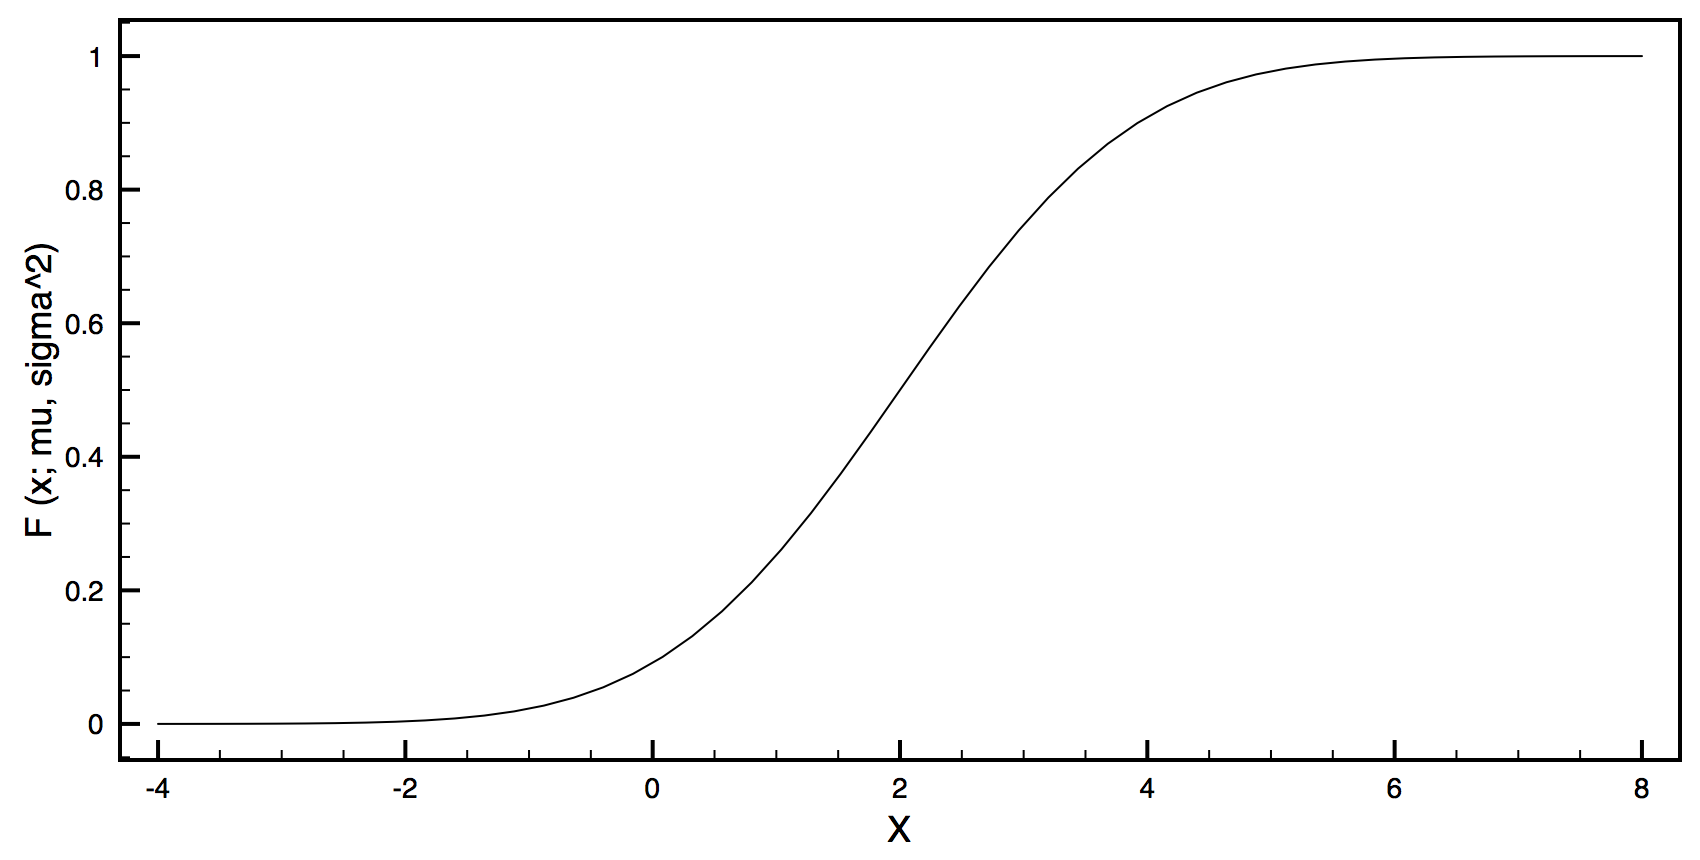
\includegraphics[width=1.\textwidth]{NCDF.png}
	\end{figure}  
It should be noted that the graph above has been bounded between -4, 8 to show symmetry, and $\sigma$ = 1.5 $\mu$ = 2. The graph obtained also agrees heavily with modern resources. What has been gained is a standard continuous distribution for some system where the cumulative density function asymptotically approaches 1, while giving the area below the curve of the probability density function.  Lastly the goal to graph the normal cumulative was reached through implementation of multiple \textbf{contains} commands, and the complex series of continued fractions, was reached successfully.        
\newpage
\begin{thebibliography}{}
 \bibitem{1}
	Z.~Papp and A.~Bill, {\it Computational Physics Lecture Notes}, California State University Long Beach.

\end{thebibliography}




\end{document}








